%\documentstyle[epsf,twocolumn]{jarticle}       %LaTeX2e仕様
\documentclass[twocolumn]{jarticle}     %pLaTeX2e仕様(platex.exeの場合)
% \documentclass[onecolumn]{ujarticle}   %pLaTeX2e仕様(uplatex.exeの場合)
%%%%%%%%%%%%%%%%%%%%%%%%%%%%%%%%%%%%%%%%%%%%%%%%%%%%%%%%%%%%%%
%%
%%  基本バージョン
%%
%%%%%%%%%%%%%%%%%%%%%%%%%%%%%%%%%%%%%%%%%%%%%%%%%%%%%%%%%%%%%%%%
\setlength{\topmargin}{-45pt}
%\setlength{\oddsidemargin}{0cm}
\setlength{\oddsidemargin}{-7.5mm}
%\setlength{\evensidemargin}{0cm}
\setlength{\textheight}{24.1cm}
%setlength{\textheight}{25cm}
\setlength{\textwidth}{17.4cm}
%\setlength{\textwidth}{172mm}
\setlength{\columnsep}{11mm}

%\kanjiskip=.07zw plus.5pt minus.5pt


% 【節が変わるごとに (1.1)(1.2) … (2.1)(2.2) と数式番号をつけるとき】
%\makeatletter
%\renewcommand{\theequation}{%
%\thesection.\arabic{equation}} %\@addtoreset{equation}{section}
%\makeatother

%\renewcommand{\arraystretch}{0.95} 行間の設定
%%%%%%%%%%%%%%%%%%%%%%%%%%%%%%%%%%%%%%%%%%%%%%%%%%%%%%%%
%\usepackage{graphicx}   %pLaTeX2e仕様(\documentstyle ->\documentclass)
\usepackage[dvipdfmx]{graphicx}
\usepackage{subcaption}
\usepackage{multirow}
\usepackage{amsmath}
\usepackage{url}
\usepackage{ulem}
\usepackage{algorithm}
\usepackage{algorithmic}
\usepackage{listings} %,jlisting} %日本語のコメントアウトをする場合jlistingが必要
%ここからソースコードの表示に関する設定
\lstset{
  basicstyle={\ttfamily},
  identifierstyle={\small},
  commentstyle={\smallitshape},
  keywordstyle={\small\bfseries},
  ndkeywordstyle={\small},
  stringstyle={\small\ttfamily},
  frame={tb},
  breaklines=true,
  columns=[l]{fullflexible},
  numbers=left,
  xrightmargin=0zw,
  xleftmargin=3zw,
  numberstyle={\scriptsize},
  stepnumber=1,
  numbersep=1zw,
  lineskip=-0.5ex
}
%%%%%%%%%%%%%%%%%%%%%%%%%%%%%%%%%%%%%%%%%%%%%%%%%%%%%%%%
\begin{document}

	%bibtex用の設定
	%\bibliographystyle{ujarticle}

	\twocolumn[
		\noindent
		\hspace{1em}
		2020 年 7 月 13 日
		発表資料
		\hfill
		B4 杉山 竜弥
		\vspace{2mm}

		\hrule
		\begin{center}
			{\Large \bf 進化的手法に基づく深層学習の構築に関する研究}
		\end{center}
		\hrule
		\vspace{9mm}
	]

  % 背景
  % 要素技術
  % 実験目的
  % 実験方法
  % 4p?
  % slackで連絡

  % 進化的な深層学習の構築に関する研究
  % AutoML
  % NAS
  % DataAugment
  %
  % DataAugment | NN, SVM, RF(包括的)
  %
  % DataAugment 最後の方の実験結果
  %
  % (進化的な人工知能の構築に関する研究)

\section{はじめに}

近年, 機械学習の発展は目覚ましく, 広範な分野に適用され多くの研究がなされている.
例えば深層ニューラルネットワーク(deep neural network; DNN)を用いた深層学習では, 音声・画像・自然言語を対象とした問題で既存(?)手法を大きく上回る高い性能を示し, 強い関心を集めた.

一方でDNNは言葉通り層を深く重ねるため, 層の種類, パラメータ, 数, 層同士の接続など多数のハイパーパラメータを持つ.
このため問題に合わせて適切なパラメータを選択しなければ良好な精度が出ないが, そのネットワークやアーキテクチャの設計に明確な指針はなく試行錯誤的にする必要があった.

この問題を解決するために自動化された機械学習(Automated Machine Learning; AutoML)と呼ばれる分野が注目されている. AutoMLではアーキテクチャ全体を対象とした最適化を目指す.
本研究ではAutoMLを用いる前段階として, 論文を紹介する. まずAutoMLの分類を見た後, その例であるNeural Architecture Search(NAS)とAuto Augmentについて示す.
また予備的に実施した数値実験についても示す.
% 本研究ではAutoMLの調査を行い, その分類と例をまとめる.

\section{要素技術}
\subsection{AutoML}
自動化された機械学習(Automated Machine Learning; AutoML)\cite{SurveyAutoML}は特定の技術ではなく, 機械学習モデルの設計を自動化する全般的な手法, または概念を指す.

問題ごとにパラメータを適切に設定する必要があるというパラメータ設定問題の解決を目的とする.
確率的なブラックボックスメタ最適化であるこの問題の解決によって,
\begin{itemize}
  \item 時間コストの削減・性能の向上
  \item アルゴリズムの評価, 比較のためパラメータの最適性の影響を緩和
  \item パラメータが与える影響の知識の必要性を排除
\end{itemize}
の3つの利益が得られる.

AutoMLはそのアルゴリズムによって, 以下の3つの主要カテゴリと5つのサブカテゴリに分類される\cite{SurveyAutoML}.

\paragraph{主要カテゴリ}
構造や構成による分類
\begin{enumerate}
  \item 単純な生成・評価法 \\
  生成段階で候補となる設定を生成, 評価段階で評価して最適な設定を見つける手法.

  \item 反復的生成・評価法 \\
  少数の設定を生成して, 最も優れたものを発見し, 反復的に生成する新しい設定の指針とする手法.

  \item 高レベルの生成・評価方法 \\
  高レベル生成機構として既存の自動パラメータ調整手法や探索手法を持ち,
  少数精鋭の設定を生成し評価段階では慎重に評価する手法.
\end{enumerate}

\paragraph{サブカテゴリ}
評価方法による分類
\begin{enumerate}
  \item 繰り返し評価法 \\
  複数回の評価を, 平均するなど統計的に評価する手法.

  \item F-Racing \\
  統計的に劣る評価の設定を段階的に排除し, 有望な候補に計算を集中する手法. 繰り返し評価より効率的になる.

  \item インテンシフィケーション(強化) \\
  問題のリストで候補設定と暫定設定の評価を次々比較し, 劣る場合は途中で排除し, そうでなければ候補が暫定設定となる手法.

  \item シャープニング \\
  少ないテスト数で評価を始め, 将来性のある設定のテスト数を2倍にすることで素早く探索できる手法.

  \item アダプティブキャッピング  \\
  有望でない設定の実行を中断して計算量を削減できる手法.
\end{enumerate}

\subsection{Neural Architecture Search}
% AutoMLの一種
従来の機械学習では手作業によって設計されたモデルをデータセットで学習して重みの最適化を行うが, アーキテクチャの設計には, 高度な専門知識と手作業による構築が必要である.
Neural Architecture Search(NAS)\cite{DBLP:journals/corr/ZophL16}は, ニューラルネットワークのアーキテクチャ自体を最適化する.

% 最適化のためまずアーキテクチャを, レイヤーの種類やその接続を表すハイパーパラメータで表現する.

アーキテクチャの探索には3つの段階がある.
まず最初にコントローラと呼ばれる再帰型ニューラルネットワーク(Recurrent Neural Network; RNN)で, アーキテクチャのハイパーパラメータを生成する.
例えば畳み込み層を利用するネットワークでは, レイヤーごとにフィルタの高さ・幅, ストライドの高さ・幅, フィルタ数が必要となる.
次にハイパーパラメータから子ネットワークを構築し, 通常のように重みを訓練して検証データセットの精度を得る.
最後に得られた精度で報酬を計算し, 方策勾配法(Policy gradient method)によってコントローラのネットワークを更新する.
これらの手順を繰り返すことで, 子ネットワークのアーキテクチャが最適化される.
% 方策勾配法:Policy(=ネットワーク)の勾配と価値関数の積を報酬として更新
% 最良の子ネットワークがコントローラが見つけたアーキテクチャとなる.

NASでは子ネットワークとして, 畳み込みネットワークとRNNを探索をし従来のネットワークより高い精度と少ないパラメータ数を達成したが, 数百台のGPUと1ヶ月の時間がかかり計算量に問題があった.
以降の研究では計算量の削減を目的とした手法が提案された.

佐藤ら\cite{ANAS}の研究では, NASを改良した先行研究と比較して, より高速なアーキテクチャ探索アルゴリズムを開発した.

特徴としてコントローラで生成していたカテゴリカルなアーキテクチャパラメータから,
アーキテクチャを確率分布で連続的に表現し, 分布推定を行う手法に変えることで, 微分可能となった.
これによって貢献度と呼ぶアーキテクチャの構成要素ごとの評価を導入して, 一様な更新ではなく構成要素ごとの勾配で更新をすることができ, 高速化ができた.

またNASではアーキテクチャ候補ごとに重みを学習し直していたが, ネットワークの重みを再利用することで大幅な学習時間の削減を達成した.

% ここはもっと詳しく説明する!!!!!!!!
\paragraph{重みの再利用}
\begin{enumerate}
  \item 冗長にネットワーク構造を決めておく. (あるノードはそれ以前のノード全てに接続可能とする)
  \item 重みを学習して、各エッジ、各演算子ごとに重みを保存
  \item アーキテクチャ(接続するか?+演算子)を探索
\end{enumerate}


\subsection{AutoAugment}

NASに対してデータセットを対象としたAutoMLも提案されている.
画像識別問題で利用されるデータセットでは, 画像データの左右反転や回転, 色相や輝度の操作することでデータ数を増やすデータ拡張(Data Augmentation; DA)が精度の向上に効果的であることが分かっている.
しかし操作の種類と強度, 操作の順序の組合せは膨大であり, 現在データ拡張の実装は手動で設計されているため試行錯誤に時間がかかる.
AutoMLの一つであるAuto Augment\cite{DBLP:journals/corr/abs-1805-09501}はデータ拡張の空間を探索し, 最高の検証精度となる最適な方策を見つける.
% 実験の内容に合わせて加筆すること!

\section{実験}
% +結果
% 本実験ではx 本研究ではo
% 1p
今回は計算時間の関係から2.3で述べたAuto Augmentについて実験をした.
Auto Augmentはデータセットを対象とした操作を最適化するが,
データセットの持つ特徴を解析する実験として, 次の予備実験をした.

以下では, 画像データの分類問題を考える.
異なるクラスラベルを持つサブデータセット集合と, それらを1つに結合したデータセットを作成する.
集合内の各サブデータセットで学習した各分類器を用いて, 結合したデータセット全体のクラス分類をする.

関連手法として, 複数のネットワークの多数決をとり1つの識別器を構成するアンサンブル学習がある
% が, データセットとクラスが固定されている点で異なる.

\subsection{データセット}
データセットは, 10クラスの画像データが含まれるCifar-10\cite{cifar10}を利用した.
サブデータセットは, Cifar-10から10クラスの内いくつかを抜き出し作成した.

\subsection{モデルの構築}
% cifar10\cite{cifar10}
% 前回, 5クラス識別器を2つ利用したモデルの構築をしたが, 10クラスの識別が50\%であったため, より適したパラメータを探索し, 再び実験して精度の向上を目指した.
分類器には, 16層の畳み込みニューラルネットワーク(Convolutional Neural Network; CNN)を用いた.
実験1では作成したサブデータセットで, 5クラス分類を学習した後, 同様に学習した他のネットワークと組合せて10クラス分類をする. 図\ref{fig:model}にこの関係を示した.

\begin{table}[tb]
  \begin{center}
    \caption{実験の設定}
    \begin{tabular}{|c|c|} \hline
      Optimizer & SDG \\ \hline
      momentum & 0.9 \\ \hline
      lr & 0.001 \\ \hline
      Loss & Cross Entropy Loss \\ \hline
      batch size & 64 \\ \hline
      epoch & 100 \\ \hline
    \end{tabular}
    \label{tab:setting}
  \end{center}
\end{table}

\begin{figure*}[t]
	\begin{center}
		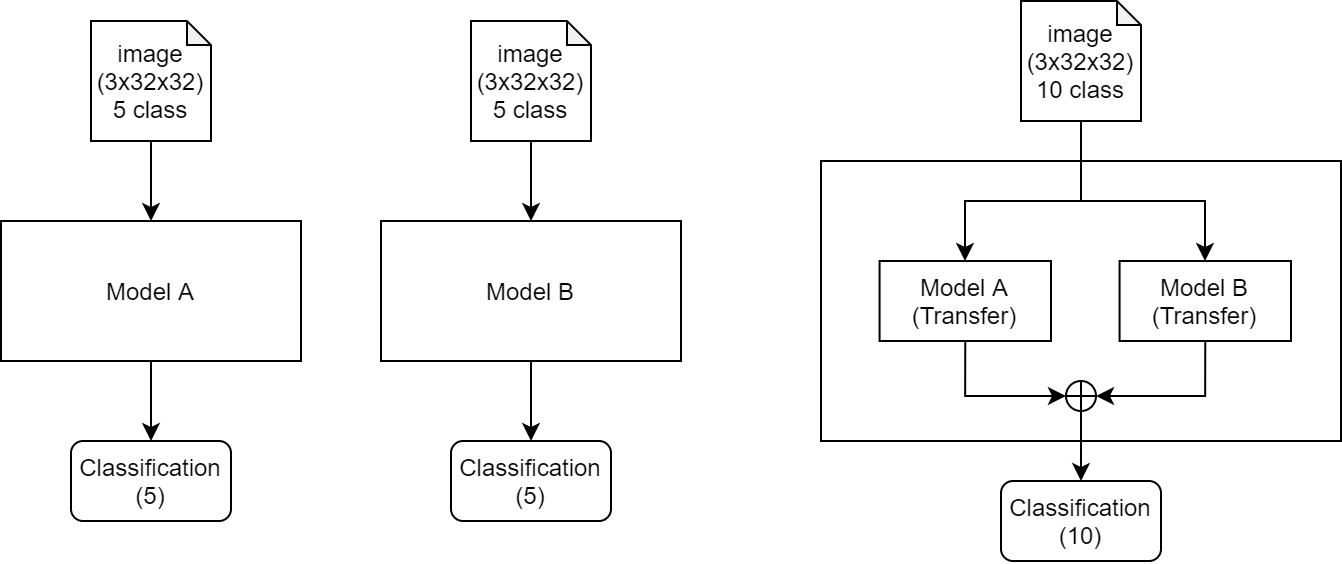
\includegraphics[clip,width=16cm]{model_figure.png}
		\caption{モデルの簡略図 ()内はデータの次元数}
		\label{fig:model}
	\end{center}
\end{figure*}

\subsection{実験1}

% 結合モデルA + Bは10クラスのデータセットをA, Bに入力し、得られた出力をクラスインデックス順に結合して、出力とする。結合では特別な処理を行わず、そのままのデータを連結した.

実験1ではデータセットを2つの異なる5クラスサブデータセットに分割した.
このデータセットはそれぞれ16,000枚の画像データが含まれる.
クラスを表す番号の前半(airplane, mobile, bird, cat, deer)で学習したモデルをA,
後半(dog, frog, horse, ship, truck)で学習したモデルをBとする.

結合したモデルA + Bは, 10クラス分類問題を解く.
結合の際は10クラスのデータセットをA, Bに入力し, 得られた出力の次元を10クラスに拡張して和を求めた.

\subsubsection{結果}

\begin{figure}[tb]
	\begin{center}
		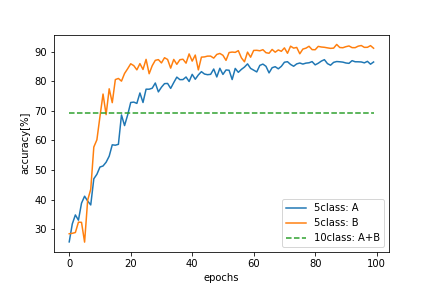
\includegraphics[clip,width=8.5cm]{accuracy5.png}
		\caption{実験1の5クラス分類器の正答率}
		\label{fig:accuracy5}
	\end{center}
\end{figure}

図\ref{fig:accuracy5}にモデルA, Bのテスト精度の結果を示した.
モデルAが84\%, Bが90\%となった. この精度はやや低いため, データ拡張による改善が望まれる.

結合モデルA + Bの10クラス分類の結果は, 70\%となった.
% ここのデータをちゃんと実験する
% 未学習のクラスは識別できないため と書く
片方のモデルのみで分類した場合, 40\%程度となるので, データセットのクラス拡張に対応していることが分かる.

\subsection{実験2}

\begin{table}[tb]
  \begin{center}
    \caption{モデルごとの7クラスの振り分け}
    \begin{tabular}{|c||c|c|c|c|c|c|c|c|c|c|} \hline
      model & 0 & 1 & 2 & 3 & 4 & 5 & 6 & 7 & 8 & 9 \\ \hline\hline
      A     & o & o & o & o & o & o & o & _ & _ & _ \\ \hline
      B     & o & o & o & o & _ & _ & _ & o & o & o \\ \hline
      C     & o & _ & _ & _ & o & o & o & o & o & o \\ \hline
    \end{tabular}
    \label{tab:class7}
  \end{center}
\end{table}

% さらに今回は, 細川君に指摘してもらったアイデアでも実験を行った. 7クラス分類器を3つ組合せて,10クラスの分類を行った. 表\ref{tab:class7}のように, 2つ以上の分類器で各クラスを推定するように, クラスを振り分けた.
あるクラスの分類を複数のモデルで実行することで, 実験1より高い精度の獲得を目指した.
7クラスを持つサブデータセットを3つ作成し, 学習するモデルをそれぞれA, B, Cとした.
各データセットのクラスは, 2つ以上の分類器でクラスを推定できるように振り分けた.
表\ref{tab:class7}には, クラスの番号と共に選択したクラスをoで示した.

\subsubsection{結果}

\begin{figure}[tb]
	\begin{center}
		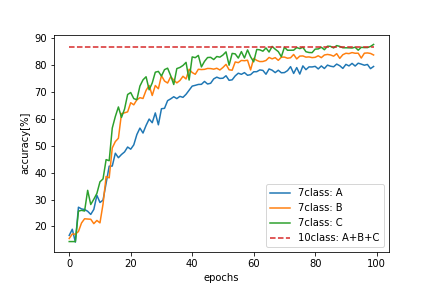
\includegraphics[clip,width=8.5cm]{accuracy7.png}
		\caption{実験2の7クラス分類器の正答率}
		\label{fig:accuracy7}
	\end{center}
\end{figure}

図\ref{fig:accuracy7}に7クラス分類の精度を示した.

7クラス分類では, 正答率が平均80\%程度で, 結合した結果10クラス分類では86.7\%となった.
クラスが増え問題が困難になっているが, 精度が高まる結果となった.

\section{考察}
% 精度が出ない,とかだけではなく自分なりの考察を示す

% なんか頑張って書く? 実験についてもっと書く?

実験1ではクラスを拡張したデータセットでの, モデルの結合の有効性を見た.
実験2では分類の結果を重ね合わせることで, テスト精度が非常に高まることが分かった.

色情報の似た画像クラスを含めることで効果的に, 形状的特徴を学習するように促すなど, データセットの統合におけるクラスの組合せに関する問題を考えたい?

図\ref{fig:accuracy5}, \ref{fig:accuracy7}ともにインデックスが前半のクラスを持つモデルでは, 正答率が低い傾向が見られた. 再度学習を行っても変わらなかったため誤差の影響ではなく, 困難なクラスの分類によって精度が下がっていると考えられる. これはクラスを単純に分割したことによる偏りに原因がある.

様々なクラスの組合せパターンで実験することで, クラスの潜在的な識別難度や, 類似クラス間の識別における相互作用などを確かめたい.
%% 分割する組合せを自由に替える実装ができたので, 様々な組合せパターンで実験して, その差異を見たい.
%% 特にモデル間の正答率の差が目立ったため, これを埋めるような組合せを探したい.

% ?????よく考えること
すべて?の組合せを進化型計算で求めるなどのAutoMLによる応用が考えられる.

\section{まとめと今後の課題}
% 論文の調査をした
% AutoMLとその関連技術についてまとめた

ネットワークによって自動的にネットワークをメタ最適化するAutoMLについて調査した.
従来では人が行っていた工程を機械学習によって自動化しようという試みがある?
一方でネットワークを複数回学習するため計算時間が問題となったが, 探索時間を削減する様々な工夫が提案された.

実験は~~であった.

今後の展望として, ~らの論文中\cite{ANAS}のモデルを再現する, ネットワークの構造を探索するNASファミリのシステムを実装し,
簡単な問題で動作実験することで, NASの理解を深めたい.
% NASについて確率的なアーキテクチャ表現したシステムを構築し
% 簡単な問題を解く小さなネットワークを探索する実験をしたい

% 参考文献リスト
\bibliographystyle{unsrt}
\bibliography{ref}
\end{document}
